\documentclass[paper=a5,pagesize=auto,twoside=false,fontsize=12pt,DIV=classic,BCOR=0mm,headinclude=true,footinclude=false]{scrbook}

%% font selection
\usepackage{utopia}
\usepackage{avant}

%% redefine headers
\usepackage[headsepline]{scrpage2}
\pagestyle{scrheadings}

\setkomafont{pageheadfoot}{%
  \normalfont\itshape
}

\automark[chapter]{chapter}
\renewcommand{\chaptermark}[1]{\markboth{#1}{#1}}
%\renewcommand{\sectionmark}[1]{\markright{#1}}

%% additional KOMA script options
\KOMAoptions{parskip=half,headsepline=true,numbers=noendperiod,captions=tableheading}
\recalctypearea{} % recalculate type area after selecting fonts

\usepackage{array}
\usepackage[british]{babel}
\usepackage{bbding}
\usepackage{float}  % direct positioning of floats
\usepackage{graphicx}
\usepackage{ifpdf}
\usepackage[utf8x]{inputenc}
\usepackage{paralist}
\usepackage{ucs}
\usepackage[obeyall]{siunitx}
\usepackage[hyphens]{url}
\usepackage{varioref}
\usepackage{wrapfig}  % must be included after package "float"

%% Make sure "hyperref" comes last of your loaded packages, to give it
%% a fighting chance of not being over-written, since its job is to
%% redefine many LATEX commands.
\ifpdf
	\usepackage[unicode,pdftex]{hyperref}
\else
	\usepackage[unicode,hypertex]{hyperref}
\fi

\hypersetup{
  unicode=true,                % non-Latin characters in Acrobat’s bookmarks
  pdftitle=K-Meter,            % title
  pdfauthor=Martin Zuther,     % author
  pdfsubject=K-Meter,          % subject of the document
  pdfcreator=Martin Zuther,    % creator of the document
  colorlinks=true,             % false: boxed links; true: colored links
  linkcolor=blue,              % color of internal links
  citecolor=blue,              % color of links to bibliography
  filecolor=blue,              % color of file links
  urlcolor=blue                % color of external links
}

%% KOMA script captions
\addtokomafont{caption}{\small}
\addtokomafont{captionlabel}{\bfseries}
\setcapindent{0em}

%% taken from package "l2tabu"
\tolerance 1414
\hbadness 1414
\emergencystretch 1.5em
\hfuzz 0.3pt
\widowpenalty=10000
\vfuzz
\hfuzz
\raggedbottom

%% package "varioref"
\labelformat{chapter}{chapter~#1}
\labelformat{section}{section~#1}
\labelformat{subsection}{section~#1}
\labelformat{subsubsection}{section~#1}

\labelformat{figure}{figure~#1}
\labelformat{table}{table~#1}

%% package "paralist"
\setdefaultitem{\textbullet}{$\circ$}{}{}

%% package "url"
\urlstyle{rm}

%% package "wrapfig"
\setlength{\intextsep}{0.2\baselineskip}

%% package "siunitx"
\sisetup{per=slash,trapambigfrac,locale=UK}

\newunit[unitspace=space]{\dB}{dB}
\newunit[unitspace=space]{\dBFS}{dB\,FS}
\newunit[unitspace=space]{\dBSPL}{dB\,SPL}
\newunit[unitspace=space]{\LK}{LK}
\newunit[unitspace=space]{\LKFS}{LK\,FS}

%% scaling of screenshots
\newcommand{\screenshotscale}{0.7}

%% layout
\usepackage[inner=18mm,outer=18mm,top=26mm,bottom=27mm,headsep=6.5mm,headheight=5mm]{geometry}

% %% start new page for every section
% \let\stdsection\section  
% \renewcommand\section{\newpage\stdsection}

%% command "application"
\DeclareRobustCommand*{\application}[1]{\texttt{#1}}


%%% Local Variables:
%%% mode: latex
%%% mode: outline-minor
%%% TeX-command-default: "Rubber"
%%% TeX-master: "../kmeter"
%%% TeX-PDF-mode: t
%%% ispell-local-dictionary: "british"
%%% End:

\hyphenation{
}


\title{K-Meter}
\author{Martin Zuther}

\begin{document}

\title{K-Meter}

\subtitle{
  \normalsize{\textrm{\textmd{
        \vfill
        Free implementation of a K-System meter \\
        according to Bob Katz' specifications
        \vfill
        \vspace{1.5em}
        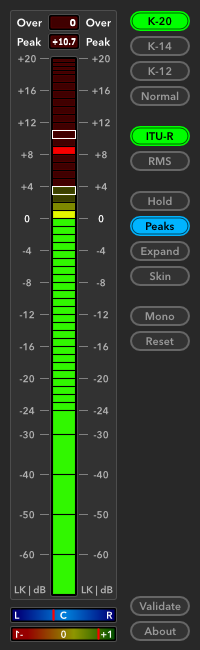
\includegraphics[scale=0.30,clip]{include/images/kmeter.png}
        \vfill
      }}}
}

\author{}

\date{\emph{Last edited on \today}}

\dedication{
  
\includegraphics[scale=0.65,clip]{include/images/cc-by-sa.png}
  \vspace{0.25em}

  This documentation by \href{http://www.mzuther.de/}{Martin Zuther}
  is licensed under a
  \href{http://creativecommons.org/licenses/by-sa/4.0/}{Creative
    Commons Attribution-ShareAlike 4.0 International License} with the
  exception of the GPL, VST and ASIO logos.
}

\maketitle

\tableofcontents

\clearpage  % layout

\chapter{The loudness race}
\label{chap:loudness_race}

When comparing two similar pieces of music, the louder one is
perceived as sounding better (although this is only true for very
short periods of time).  Accordingly, the loudness of music
productions has continuously grown during the last decades.

As maximum levels of records, tapes and digital media have a natural
limit, however, mastering engineers have started using sophisticated
dynamic compression techniques to achieve higher loudness without
distorting the music (as of 2010, distortion is increasingly being
used in order to achieve even higher loudness).

Unfortunately, this decrease in dynamic range does not leave the music
unharmed.  Current compressed music blasts away your ears and makes
you turn down the volume of your amplifier.  Having lowered the
volume, you'll find that the ``better-sounding'' compressed music
suddenly sounds pretty dull and boring compared to uncompressed music.
In contrast, music with high dynamic range makes you turn up the
volume -- heck, it even sounds better when being broadcast on the
radio!

\chapter{The K-System}
\label{chap:k_system}

The K-System has been devised by mastering engineer Bob Katz in order
to counteract the ongoing loudness race and to help adjusting the
levels of different songs during mastering.  K-System meters are level
meters that do \textbf{not} place the \SI{0}{\dB} mark on top of the
meter.  Instead, \SI{0}{\dB} on K-System meters relates to a reference
loudness.  There are three K-System scales:

\begin{compactitem}
\item K-20 (\SI{0}{\dB} at \SI{-20}{\dBFS}, recommended)
\item K-14 (\SI{0}{\dB} at \SI{-14}{\dBFS})
\item K-12 (\SI{0}{\dB} at \SI{-12}{\dBFS})
\end{compactitem}

Using the K-System is easy.  Just calibrate your monitor system so
that pink noise (\SI{-20}{\dBFS}\,RMS, \SI{20}{\hertz} to
\SI{20}{\kilo\hertz}; \ref{chap:validation} will tell you where to
find a suitable audio file) on one channel yields \SI{83}{\dBSPL} on a
loudness meter placed at your listening position and set to
\emph{C-weighted, slow}.  Then mark the monitor's gain position as
``K-20''.

When your mixes or masters seem to have just the right loudness, they
should now yield \SI{0}{\dB} on a K-20 meter.

In case you want to use the K-14 meter, attenuate the monitor gain by
\SI{6}{\dB} or repeat the above process so that pink noise yields
\SI{77}{\dBSPL}.  For K-12, attenuate the monitor gain by another
\SI{2}{\dB} (pink noise should yield \SI{75}{\dBSPL}).

For more information about the K-System, please see
\href{http://www.digido.com/level-practices-part-2-includes-the-k-system.html}{Bob's
  website} or his great book ``Mastering Audio -- The Art and the
Science (second edition)''.

\chapter{Installation}
\label{chap:installation}

In order to use the pre-compiled binaries, simply extract the K-Meter
files from the downloaded archive.  For the plug-ins, you'll then have
to move the extracted files to your respective plug-in folder
(\path{~/.lv2}, \path{~/.vst}, \path{C:\Program
  Files\Steinberg\VstPlugins\} or the like).

Loading K-Meter may take a few seconds: it checks your computer's
capabilities on start-up so that FFT calculations will run at maximum
speed.  Depending on your computer, this little wait in the beginning
may well result in lower resource usage later.

Should the standalone version ever fail to start, you can reset its
settings by deleting the file \path{kmeter_stereo.ini} or
\path{kmeter_surround.ini}.  These files are located in
\path{~/.config} (GNU/Linux) or \path{%appdata%\.config\} (Windows).

\chapter{Controls}
\label{chap:controls}

\section{Meter selection}

\begin{wrapfigure}{r}{0pt}
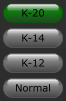
\includegraphics[scale=\screenshotscale,clip]{include/images/button_meter_selection.png}
\end{wrapfigure}

You can select the different K-System meter scales (\textbf{K-20},
\textbf{K-14} and \textbf{K-12}) by clicking on these radio buttons.
In the rare case that you want to use the meter in a mixer's channel
strip, click the \textbf{Normal} button which will place \SI{0}{\dBFS}
on top of the meter's scale.

\begin{wrapfigure}{r}{0pt}
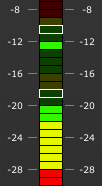
\includegraphics[scale=0.60,clip]{include/images/kmeter_normal_scale.png}
\end{wrapfigure}

The \textbf{Normal} scale looks a little different.  It has been
designed for gain staging during recording: average levels should stay
in the lower green area (and thus below \textbf{\SI{-18}{\dBFS}}),
while peak levels should not exceed the upper yellow bar
(\textbf{\SI{-9}{\dBFS}}).  However, you may find my latency-free
plug-in \href{http://code.mzuther.de/}{\textbf{traKmeter}} better
suited for gain staging.

\newpage %% layout

\section{Averaging method}

\begin{wrapfigure}{r}{0pt}
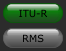
\includegraphics[scale=\screenshotscale,clip]{include/images/button_averaging_selection.png}
\end{wrapfigure}

The average level meters can either read unweighted levels
(\textbf{RMS}) or loudness-weighted levels according to
\href{http://www.itu.int/rec/R-REC-BS.1770}{ITU-R BS.1770-1}
(\textbf{ITU-R}).  Click on the corresponding radio button to make
your selection.

According to Bob Katz, the unweighted \textbf{RMS} method has been
designed for stereophonic metering and calibration, while the
loudness-weighted \textbf{ITU-R} method should be used for
channel-summed loudness metering.  To reference a meter, state both
K-System meter scale and averaging method, separated by a slash, such
as ``K-20/ITU-R''.

\emph{\underline{Note:} K-Meter fully implements Annex 1 of the now
  superseded ITU-R BS.1770-1 standard ('K' frequency weighting, mean
  square calculation and channel-weighted summation), whereas the
  gated loudness measurement specified in ITU-R BS.1770-4 is not
  supported.}

\section{Infinite peak hold}

\begin{wrapfigure}{r}{0.14\linewidth}

\includegraphics[scale=\screenshotscale,clip]{include/images/button_peak_hold_on.png}
\newline \vspace{-0.9\baselineskip}

\includegraphics[scale=\screenshotscale,clip]{include/images/button_peak_hold_off.png}
\end{wrapfigure}

Click on this button to toggle between infinite peak hold and
``falling peaks''.  This setting applies to both average and peak
meters.

\section{Show peak level meter}

\begin{wrapfigure}{r}{0.14\linewidth}

\includegraphics[scale=\screenshotscale,clip]{include/images/button_peak_meter_on.png}
\newline \vspace{-0.9\baselineskip}

\includegraphics[scale=\screenshotscale,clip]{include/images/button_peak_meter_off.png}
\end{wrapfigure}

Click on this button to toggle display of the peak level meters.  The
original K-System meter specification demands peak level meters, but
Bob Katz has asked me to hide them by default:

\begin{quotation}
  \emph{``Too many people will try to normalize the peak to full scale
    if they see a peak meter, and that's what we want to avoid.  You
    can still make a K-System meter like the original, but if we meet
    again in \num{15} years I hope that peak metering will be
    outlawed.''}
\end{quotation}

\section{Discrete segments}

\begin{wrapfigure}{r}{0.14\linewidth}

\includegraphics[scale=\screenshotscale,clip]{include/images/button_discrete_on.png}
\newline \vspace{-0.9\baselineskip}

\includegraphics[scale=\screenshotscale,clip]{include/images/button_discrete_off.png}
\end{wrapfigure}

This button switches between the discrete meters that are used on
analogue gear and the continuous meters typically found in DAWs.

\section{Magnify meters}

\begin{wrapfigure}{r}{0.14\linewidth}

\includegraphics[scale=\screenshotscale,clip]{include/images/button_expand_meter_on.png}
\newline \vspace{-0.9\baselineskip}

\includegraphics[scale=\screenshotscale,clip]{include/images/button_expand_meter_off.png}
\end{wrapfigure}

This button magnifies both average and peak level meters to
\SI{0.1}{\dB} steps.  If switched on, the \SI{0}{\dB} mark (normal
scale: \SI{-22}{\dB} mark) is placed near the meter's bottom.

\newpage %% layout

\section{Mono mode}

\begin{wrapfigure}{r}{0.14\linewidth}

\includegraphics[scale=\screenshotscale,clip]{include/images/button_mono_on.png}
\newline \vspace{-0.9\baselineskip}

\includegraphics[scale=\screenshotscale,clip]{include/images/button_mono_off.png}
\end{wrapfigure}

Click this button to easily check the mono compatibility of your
stereo mix or master.  In \textbf{mono} mode, audio channels will be
down-mixed to mono and the meters will be linked.

If you insert the stereo plug-in into a mono channel strip,
\textbf{mono} mode will be selected and cannot be toggled.  In the
surround version, the \textbf{mono} button is disabled.

\section{Reset button}

\begin{wrapfigure}{r}{0.14\linewidth}

\includegraphics[scale=\screenshotscale,clip]{include/images/button_reset_on.png}
\newline \vspace{-0.9\baselineskip}

\includegraphics[scale=\screenshotscale,clip]{include/images/button_reset_off.png}
\end{wrapfigure}

Click on this button to reset all meters.  You can also use it to get
rid of graphical artefacts, because the current skin will be reloaded
and all meters redrawn.

\section{Select a skin}

\begin{wrapfigure}{r}{0.14\linewidth}

\includegraphics[scale=\screenshotscale,clip]{include/images/button_skin_on.png}
\newline \vspace{-0.9\baselineskip}

\includegraphics[scale=\screenshotscale,clip]{include/images/button_skin_off.png}
\end{wrapfigure}

Click on this button to select a new K-Meter skin.  You can also set a
default skin that will be loaded when new plug-ins are instantiated.

\newpage %% layout

\section{Validation button}
\label{sec:validation_button}

\begin{wrapfigure}{r}{0.14\linewidth}

\includegraphics[scale=\screenshotscale,clip]{include/images/button_validate_on.png}
\newline \vspace{-0.9\baselineskip}

\includegraphics[scale=\screenshotscale,clip]{include/images/button_validate_off.png}
\end{wrapfigure}

Click on this button to open the \textbf{validation window} (see
\ref{chap:validation}) which allows you to play an audio file through
K-Meter and dump internal data.  During validation, the button will
light up and clicking it will stop validation early.

\emph{Unfortunately, the underlying JUCE library does not seem to
  support multi-channel audio files.  You may load such audio files
  into your DAW of choice and use a K-Meter plug-in.}

On Linux, dumped data will be written to \path{stderr}, so just start
the K-Meter standalone or your VST host from the shell and watch the
output coming.  On other systems, have a look at your VST host's log
files (I have successfully used Ableton Live for this).  If that
doesn't work, you might have to start either the K-Meter standalone or
your VST host from a debugger.

As a side note, \textbf{SMA(50)} designates the simple moving average
of 50 values, a neat way to emphasise trends and eliminate short-term
fluctuations.

\section{About button}

\begin{wrapfigure}{r}{0.14\linewidth}

\includegraphics[scale=\screenshotscale,clip]{include/images/button_about_on.png}
\newline \vspace{-0.9\baselineskip}

\includegraphics[scale=\screenshotscale,clip]{include/images/button_about_off.png}
\end{wrapfigure}

Clicking on this button will open the \textbf{about window} where you
will be informed about version number, contributors, copyright and the
GNU General Public License.

\section{Display license}

\begin{wrapfigure}{r}{0.15\linewidth}

\includegraphics[scale=\screenshotscale,clip]{include/images/button_gpl_on.png}
\newline \vspace{-0.9\baselineskip}

\includegraphics[scale=\screenshotscale,clip]{include/images/button_gpl_off.png}
\end{wrapfigure}

This button is located in the \textbf{about window} and does not only
advertise that you are using free software licensed under the
\textbf{GNU General Public License} -- when clicked, it will also open
the license's website in your web browser \dots

\chapter{Meters}
\label{chap:meters}

For \num{5.1} surround sound, K-Meter assumes a channel order of
\emph{L}, \emph{R}, \emph{C}, \emph{LFE}, \emph{Ls} and \emph{Rs}.
Please double-check whether this matches your host's channel order.

\section{K-System meter}

\begin{wrapfigure}{r}{0.19\linewidth}
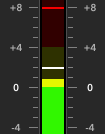
\includegraphics[scale=0.58,clip]{include/images/level_meter_itu_continuous.png}
\newline \vspace{-0.55\baselineskip}
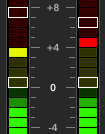
\includegraphics[scale=0.58,clip]{include/images/level_meter_rms_discrete.png}
\end{wrapfigure}

The K-System meter consists of an average level meter (coloured bar)
and an optional peak level meter (single coloured segment).  The
recommended K-20 scale has \SI{20}{\dB} of headroom above \SI{0}{\dB},
while the K-14 and K-12 scales have \SI{14}{\dB} and \SI{12}{\dB} of
headroom, respectively.

Each level meter is divided into steps of \SI{1}{\dB}, with the
exception of the top \SI{2}{\dB} (steps of \SI{0.5}{\dB}) and the
non-linear bottom end.  Magnified level meters are divided into steps
of \SI{0.1}{\dB}.

\emph{\underline{Note:} In ITU-R mode, the average level meter is
  graded in \emph{\si{\LK}} which stands for \emph{Loudness, K
    weighted} and is by all means equivalent to \si{\dB}.}

Recent maximum levels are displayed by white bars.  Unless ``Infinite
peak hold'' is switched on, maximum levels are held for
\SI{10}{\second} and then start falling with a fall time of
\SI{8.67}{\dB\per\second}.

Both stand-alone application and the plug-in only work at sampling
rates between \SI{44.1}{\kilo\hertz} and \SI{192}{\kilo\hertz} and
introduce a latency of \num{1024} samples.  This latency is reported
to your plug-in host so it may compensate for the introduced delay.
Needless to say, the original unfiltered signal is passed to the
outputs.

You can reset all meters by clicking on the ``Reset'' button.

\section{Average level meter}

The average level meter uses an averaging period of \num{1024}
samples.  In \textbf{RMS} mode, this meter exhibits a flat frequency
response between \SI{20}{\hertz} and \SI{20}{\kilo\hertz} (\SI{\pm
  0.01}{\dB}), whereas \textbf{ITU-R} mode implements 'K' frequency
weighting and also sums all channels as specified in
\href{http://www.itu.int/rec/R-REC-BS.1770}{ITU-R BS.1770-1}.

In all modes, the average level meter is band-limited using a
windowed-sinc low-pass filter with a cutoff frequency of
\SI{21.0}{\kilo\hertz}.  On level changes, it takes
\SI{600}{\milli\second} for the meter to reach \SI{99}{\percent} of
the final reading.

\emph{\underline{Note:} Unfortunately, the specifications of ITU-R
  BS.1770-1 clash with those for K-System meters.  I have discussed
  this in depth with Bob Katz and we decided that it makes more sense
  to adhere to ITU-R BS.1770-1 in these cases.}

\emph{Thus, in ITU-R mode sine waves do \emph{not} read the same on
  average and peak level meters.  Moreover, pink noise
  (\SI{-20}{\dBFS}\,RMS, \SI{20}{\hertz} to \SI{20}{\kilo\hertz}) does
  \emph{not} read \SI{0}{\dB} on the K-20 average level meter.
  \textbf{So for calibration, please switch K-Meter to RMS mode!}}

\section{Peak level meter}

The peak level meter displays the unfiltered peak level and thus
possesses a completely flat frequency response.  It has a rise time of
one sample and a fall time of \SI{8.67}{\dB\per\second}.

\emph{Please note that this meter does not register inter-sample
  peaks.}

\section{Overload counter}

\begin{wrapfigure}{r}{0.23\linewidth}

\includegraphics[scale=\screenshotscale,clip]{include/images/overload_counter_normal.png}
\newline

\includegraphics[scale=\screenshotscale,clip]{include/images/overload_counter_clipped.png}
\end{wrapfigure}

The overload counter displays the number of samples that have reached
or exceeded digital full scale (to be exact, the counter registers
levels above \SI{-0.001}{\dBFS} to address the granularity of
\num{16}-bit floating-point numbers).

\emph{Please note that this counter does not register inter-sample
  peaks.}

\section{Maximum peak display}

\begin{wrapfigure}{r}{0.23\linewidth}

\includegraphics[scale=\screenshotscale,clip]{include/images/maximum_peak_normal.png}
\newline

\includegraphics[scale=\screenshotscale,clip]{include/images/maximum_peak_clipped.png}
\end{wrapfigure}

This meter displays the maximum peak level encountered so far in
\si{\dB}.  In case the level exceeds \SI{-0.2}{\dBFS}, the meter will
turn red.

\emph{Please note that this display does not register inter-sample
  peaks.}

\section{Phase correlation meter}

\begin{wrapfigure}{r}{0pt}

\includegraphics[scale=\screenshotscale,clip]{include/images/phase_correlation_meter.png}
\end{wrapfigure}

This meter only works for stereo channels and displays the cross
correlation between left and right channel.  Cross correlation is a
measure of how much two signals are correlated.  Thus, a value of
\num[retainplus]{+1} means that both channels are \emph{in phase},
whereas a value of \num{-1} signals that the channels are completely
\emph{out of phase}.  Please note that the meter's scale is not
linear!

For the non-tech savvy musician: if you find that this meter hits the
red area, you should check the mono-compatibility of your mix.  But
although phase correlation meters often prove helpful, you cannot
always rely on their readout.  The only way to make sure that your
mixes are mono-compatible is to actually listen to them in mono.

That's a universal truth, by the way.  Do not mix by your eyes, mix by
your ears!

\section{Stereo meter}

\begin{wrapfigure}{r}{0pt}

\includegraphics[scale=\screenshotscale,clip]{include/images/stereo_meter.png}
\end{wrapfigure}

The stereo meter obviously only works for stereo channels and displays
the average stereo position of your mix.  It may indicate a bias to
one stereo channel that you might have overheard due to impaired
hearing, wrong placement of your monitors or similar problems.

But please don't get the false notion that the needle should stay in
the middle all the time in order to achieve a good mix.  Quite the
contrary!  As I said before, you should not mix by your eyes \dots

\chapter{Validation}
\label{chap:validation}

I have gone to great lengths to ensure that all meters read correctly.
You want to validate for yourself?  Just download and extract the
source code.  The directory \path{validation} contains instructions
and FLAC-compressed wave files.  To validate \textbf{ITU-R} mode,
please download \href{http://www.itu.int/pub/R-REP-BS.2217}{ITU-R
  BS.2217-1} and follow the instructions (ignore the tests for
loudness gating).  A word of warning: these audio files may
\textbf{damage your ears} and speakers, so please watch your monitor
levels!

Begin by starting K-Meter.  If in a Bash shell, try this:

\begin{VerbatimBoth}
  ./kmeter_stereo 2>&1 | tee /tmp/validate.log
\end{VerbatimBoth}

\begin{wrapfigure}{r}{0.25\linewidth}
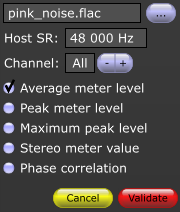
\includegraphics[scale=0.50,clip]{include/images/dialog_validation.png}
\end{wrapfigure}

After opening the \textbf{validation window} (see
\ref{sec:validation_button}), click on the ellipsis button (the one
with the dots) to select an audio file for playback through K-Meter.
Please make sure that the sample rates of your host (\textbf{Host SR})
and the audio file match, otherwise the results will not be correct.

Now, select which \textbf{variables} (if any) should be dumped.  You
may also restrict dumped data to a specific audio \textbf{channel}.
Check \textbf{CSV} if you want to feed the output to a parser.

Finally, click on the \textbf{validate} button to reset all meters and
start playback of the selected audio file.  All audio input will be
discarded during playback and for an additional twenty seconds.  To
stop playback early, simply click on the \textbf{validate} button
again.

In case you want to calibrate your monitor system, locate the file
\path{pink_noise_bandlimited.flac} in the directory \path{validation},
set K-Meter to \textbf{RMS} mode and click on the \textbf{validate}
button.  Please ensure that all intermediate software and hardware
mixers are set to the correct levels.

\newpage %% layout

\section{Validation status}

\begin{minipage}{1.0\linewidth}
  \renewcommand{\thempfootnote}{\arabic{mpfootnote}}
  \begin{tabular}{>{\bfseries}llcc}

    &
    \textbf{Readout} &
    \textbf{RMS} &
    \textbf{ITU-R} \\

    Avg level meter &
    meter ballistics &
    \Checkmark{} &
    (\Checkmark{}) \\

    &
    readings &
    \Checkmark{} &
    --- \\

    &
    frequency response &
    \Checkmark{} &
    \Checkmark{} \\

    &
    pink noise &
    \Checkmark{} &
    --- \\

    &
    ITU-R BS.2217-1 &
    --- &
    \Checkmark{} \\

    Peak level meter &
    meter ballistics &
    \Checkmark{} &
    \Checkmark{} \\

    &
    readings &
    \Checkmark{} &
    \Checkmark{} \\

    Maximum peak &
    readings &
    \Checkmark{} &
    \Checkmark{} \\

    Overload counter &
    readings &
    \Checkmark{} &
    \Checkmark{} \\

    Phase correlation &
    readings &
    \Checkmark{} &
    \Checkmark{} \\

    Stereo meter &
    readings &
    \Checkmark{} &
    \Checkmark{} \\

  \end{tabular}
\end{minipage}

\section{Frequency and phase response}

Frequency and phase response have been determined using Christan
Budde's fantastic
\href{http://www.pcjv.de/applications/measurement-programs/}{VST
  Plugin Analyser} with a sample rate of \SI{192}{\kilo\hertz} and a
log sine sweep as input signal (set using Ctrl-Shift-F).

\newpage %% layout

\textbf{Frequency response of complete effect path (\SI{5}{\hertz} to
  \SI{96}{\kilo\hertz}, \SI{0}{\dB} \SI{\pm 0.1}{\dB}):}

\begin{center}
  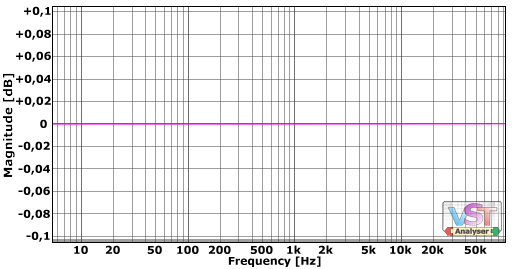
\includegraphics[scale=0.60,clip]{include/images/fft_192khz-freq-fx_path.png}
\end{center}

\textbf{Phase response of complete effect path (\SI{5}{\hertz} to
  \SI{96}{\kilo\hertz}, \SI{0}{\degree}\,\SI{\pm 0.1}{\degree}):}

\begin{center}

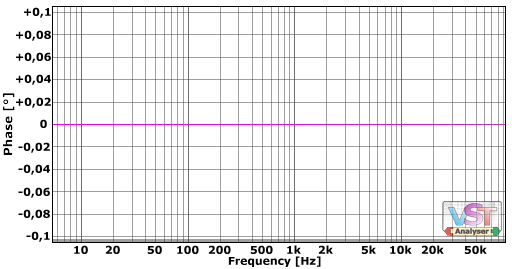
\includegraphics[scale=0.60,clip]{include/images/fft_192khz-phase-fx_path.png}
\end{center}

\textbf{Frequency response of band-limited RMS detection stage
  (\SI{5}{\hertz} to \SI{96}{\kilo\hertz}, \SI{-140}{\dB} to
  \SI{5}{\dB}):}

\begin{center}
  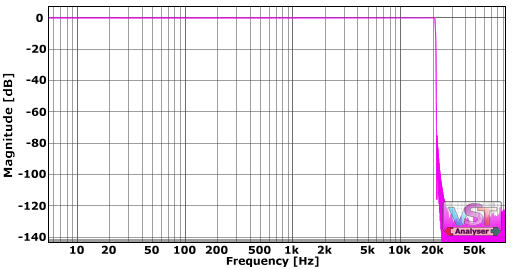
\includegraphics[scale=0.60,clip]{include/images/fft_192khz-freq-rms.png}
\end{center}

\textbf{Phase response of band-limited RMS detection stage
  (\SI{5}{\hertz} to \SI{96}{\kilo\hertz}, \SI{-180}{\degree} to
  \SI[addsign]{+180}{\degree}):}

\begin{center}
  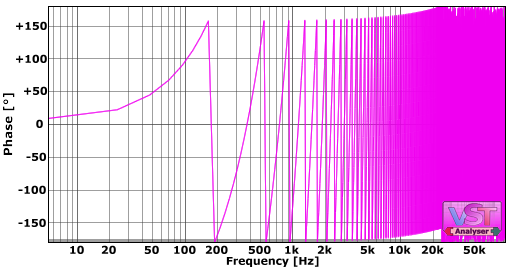
\includegraphics[scale=0.60,clip]{include/images/fft_192khz-phase-rms.png}
\end{center}
\newpage %% layout

\textbf{Frequency response of band-limited ITU-R BS.1770-1 detection stage
  (\SI{5}{\hertz} to \SI{96}{\kilo\hertz}, \SI{-140}{\dB} to
  \SI{5}{\dB}):}

\begin{center}
  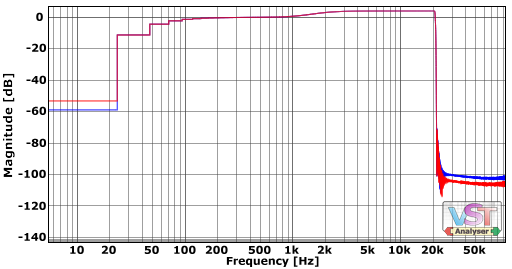
\includegraphics[scale=0.60,clip]{include/images/fft_192khz-freq-itu_r.png}
\end{center}

\textbf{Phase response of band-limited ITU-R BS.1770-1 detection stage
  (\SI{5}{\hertz} to \SI{96}{\kilo\hertz}, \SI{-180}{\degree} to
  \SI[addsign]{+180}{\degree}):}

\begin{center}
  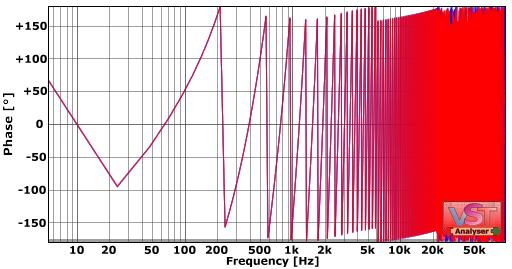
\includegraphics[scale=0.60,clip]{include/images/fft_192khz-phase-itu_r.png}
\end{center}

\newpage %% layout

\textbf{Frequency response of band-limited RMS detection stage
  (\SI{5}{\hertz} to \SI{96}{\kilo\hertz}, \SI{0}{\dB} \SI{\pm
    4}{\dB}):}

\begin{center}
  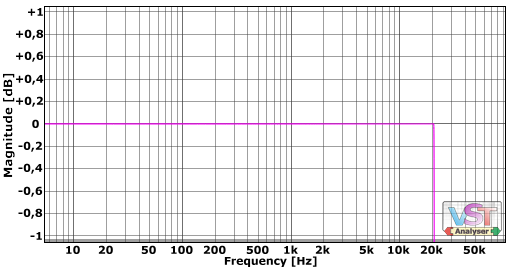
\includegraphics[scale=0.60,clip]{include/images/fft_192khz-freq_zoomed-rms.png}
\end{center}

\textbf{Frequency response of band-limited ITU-R BS.1770-1 detection stage
  (\SI{5}{\hertz} to \SI{96}{\kilo\hertz}, \SI{0}{\dB} \SI{\pm
    4}{\dB}):}

\begin{center}
  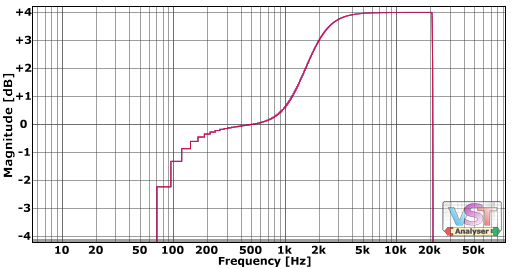
\includegraphics[scale=0.60,clip]{include/images/fft_192khz-freq_zoomed-itu_r.png}
\end{center}

\chapter{Final words}
\label{chap:final_words}

I want to express my gratitude to \textbf{Bob Katz} for kindly
answering all of my questions regarding the K-System meter and
checking this document for technical errors.  I'd further like to
thank \textbf{Tod Gentille} for creating the Mac binaries,
\textbf{bram@smartelectronix} for his code to calculate logarithmic
rise and fall times, and \textbf{Raiden} for working out the ITU-R
BS.1770-1 filter specifications.  I must also thank the \textbf{beta
  testers} and \textbf{users of K-Meter} for sending kind words,
suggestions and bug reports.  Finally, I want to thank the
\textbf{open source community} for making all of this possible.

Although coding K-Meter has been a lot of fun, it has also been a lot
of work.  So if you like K-Meter, why not send me a short email and
tell me so?  Write a few words about yourself, send suggestions for
future updates or volunteer to create a nice skin.  I also really
enjoy listening to music that you may have produced using my
software\dots

Here is my email address (please remove ``\texttt{-nospam}''):

\begin{center}
  \texttt{"Martin Zuther" <code-nospam@mzuther.de>}
\end{center}

Thanks for using free software.  I hope you'll enjoy it!

\begin{wrapfigure}{l}{0.17\linewidth}
  
\includegraphics[scale=0.40,clip]{include/images/trademark_vst.png}
\end{wrapfigure}

\emph{VST is a trademark and software of Steinberg Media Technologies
  GmbH.}

\begin{wrapfigure}{l}{0.17\linewidth}
  
\includegraphics[scale=0.60,clip]{include/images/trademark_asio.png}
\end{wrapfigure}

\emph{ASIO is a trademark and software of Steinberg Media Technologies
  GmbH.}

\appendix

\chapter{How to build K-Meter}
\label{chap:build_kmeter}

\section{Preparing GNU/Linux}

To build K-Meter yourself, I recommend setting up a \texttt{chroot}
environment.  This is fast and easy to do on Debian-based systems and
might save you a \textbf{lot} of trouble.  At the time of writing, I'm
using Linux Mint 17, but the procedure should be similar on
your distribution of choice.

Start by installing the necessary packages:

\begin{VerbatimBoth}
  sudo apt-get install debootstrap schroot
\end{VerbatimBoth}

Then install the \texttt{chroot} base system, execute the following
statements (please change \path{http://ftp.de.debian.org/debian/} to a
\href{http://www.debian.org/mirror/list}{mirror} close to you):

\begin{Verbatim32}
  sudo debootstrap --variant=buildd \
    --arch i386 stable \
    /srv/chroot/stable_i386 \
    http://ftp.de.debian.org/debian/
\end{Verbatim32}

\begin{Verbatim64}
  sudo debootstrap --variant=buildd \
    --arch amd64 stable \
    /srv/chroot/stable_amd64 \
    http://ftp.de.debian.org/debian/
\end{Verbatim64}

Running \path{debootstrap} will take some time.  Meanwhile, add the
following lines to \path{/etc/schroot/schroot.conf} (make sure you
remove all preceding white space so that each line begins in the first
column):

\begin{VerbatimBoth}
  [stable-i386]
  description=Debian stable (i386)
  directory=/srv/chroot/stable_i386
  personality=linux32
  root-users=username
  type=directory
  users=username,another_user

  [stable-amd64]
  description=Debian stable (amd64)
  directory=/srv/chroot/stable_amd64
  personality=linux
  root-users=username
  type=directory
  users=username,another_user
\end{VerbatimBoth}

Please make the necessary changes to \texttt{username}.  You may also
add additional users, like \texttt{another\_user}.  If you experience
problems, try to change \texttt{stable} to a release name such as
\texttt{wheezy}.

When \path{debootstrap} is done, log in as superuser:

\begin{Verbatim32}
  schroot -c stable-i386 -u root
\end{Verbatim32}

\begin{Verbatim64}
  schroot -c stable-amd64 -u root
\end{Verbatim64}

You'll have to install a few packages -- \path{less} and \path{vim}
are optional, but might come in handy:

\begin{VerbatimBoth}
  apt-get update
  apt-get -y install bash-completion \
    libasound2-dev libjack-jackd2-dev \
    mesa-common-dev xorg-dev less vim
  apt-get clean
\end{VerbatimBoth}

If you like \path{bash} completion, you might also want to open the
file \path{/etc/bash.bashrc} and unquote these lines:

\begin{VerbatimBoth}
  # enable bash completion in interactive shells
  if [...]
    [a couple of lines...]
  fi
\end{VerbatimBoth}

Finally, log out and log in as normal user:

\begin{Verbatim32}
  schroot -c stable-i386
\end{Verbatim32}

\begin{Verbatim64}
  schroot -c stable-amd64
\end{Verbatim64}

In this \path{chroot} shell, install the dependencies (see below).
Congratulations -- you are now ready to build K-Meter!

\section{Dependencies}

\subsection{premake}
\label{sec:dependencies_premake}

\begin{tabbing}
  \hspace*{6em}\=\=\kill

  Importance:  \> required \\
  Version:     \> 4.3 \\
  License:     \> BSD \\
  Homepage:    \> \href{http://industriousone.com/premake}{industriousone.com/premake}
\end{tabbing}

\subsubsection{Installation}

Place the binary somewhere in your \path{PATH}.  Depending on your
platform, you should run \path{premake} using the scripts
\path{Builds/run_premake.sh} or \path{Builds/run_premake.bat}.

To change the premake file using the provided Jinja templates, install
the necessary dependencies and run the Python script
\path{Builds/create_premake.py}.

\newpage %% layout

\subsection{JUCE library}

\begin{tabbing}
  \hspace*{6em}\=\=\kill

  Importance:  \> required \\
  Version:     \> 4.2.1 \\
  License:     \> ISC and GPL v3 (among others) \\
  Homepage:    \> \href{http://www.juce.com/}{www.juce.com}
\end{tabbing}

\subsubsection{Installation}

Extract the archive into the directory \path{libraries/juce}.

If you want to build the LV2 plug-in, please extract the archive
\path{distrho_lv2-xxxxxxxxxx.tar.gz} into the same directory.

\subsection{Virtual Studio Technology SDK}

\begin{tabbing}
  \hspace*{6em}\=\=\kill

  Importance:  \> optional \\
  Version:     \> 3.6.5 \\
  License:     \> proprietary \\
  Homepage:    \> \href{http://ygrabit.steinberg.de/}{ygrabit.steinberg.de}
\end{tabbing}

\subsubsection{Installation}

Just extract the archive into the directory
\path{libraries/vstsdk3.6.5}.

\subsection{Audio Streaming Input Output SDK}

\begin{tabbing}
  \hspace*{6em}\=\=\kill

  Importance:  \> optional \\
  Version:     \> 2.3 \\
  License:     \> proprietary \\
  Homepage:    \> \href{http://ygrabit.steinberg.de/}{ygrabit.steinberg.de}
\end{tabbing}

\subsubsection{Installation}

Simply extract the archive into the directory
\path{libraries/asiosdk2.3}.

\subsection{Fastest Fourier Transform in the West}

\begin{tabbing}
  \hspace*{6em}\=\=\kill

  Importance:  \> required \\
  Version:     \> 3.3.4 \\
  License:     \> GPL v2 \\
  Homepage:    \> \href{http://www.fftw.org/}{www.fftw.org}
\end{tabbing}

\subsubsection{Installation on GNU/Linux}

Extract the archive into the directory \path{libraries/fftw3}, change
into this directory and run:

\begin{Verbatim32}
  ./configure --enable-float --with-pic
  make
  mkdir -p bin/linux/i386/
  mv .libs/* bin/linux/i386/
\end{Verbatim32}

\begin{Verbatim64}
  ./configure --enable-float --with-pic
  make
  mkdir -p bin/linux/amd64/
  mv .libs/* bin/linux/amd64/
\end{Verbatim64}

\subsubsection{Installation on Mac OS X}

Extract the archive into the directory \path{libraries/fftw3}, change
into this directory and run:

\begin{Verbatim32}
  ./configure --enable-float --with-pic
  make
  mkdir -p bin/mac/x32/
  mv .libs/* bin/mac/x32/
\end{Verbatim32}

\begin{Verbatim64}
  ./configure --enable-float --with-pic
  make
  mkdir -p bin/mac/x64/
  mv .libs/* bin/mac/x64/
\end{Verbatim64}

\subsubsection{Installation on Microsoft Windows}

Extract the source code archive into the directory
\path{libraries/fftw3} and the archive containing the pre-compiled
binaries into the directory \path{libraries/fftw3/bin}.

Please note that in order to run K-Meter on Windows, the directory
\path{kmeter} containing the FFTW libraries (and skins) \textbf{must}
be located in the same directory as the standalone or plug-in.  To
make things a little easier for you, I have already placed this
directory in \path{bin} and \path{bin/final}.

\subsection{Python}

\begin{tabbing}
  \hspace*{6em}\=\=\kill

  Importance:  \> optional \\
  Version:     \> 3.4 (or higher) \\
  License:     \> Python Software Foundation License \\
  Homepage:    \> \href{http://www.python.org/}{www.python.org}
\end{tabbing}

You'll only need Python if you want to change the premake file (see
\ref{sec:dependencies_premake}) using Jinja templates or for building
\num{64}-bit versions of K-Meter using Visual Studio Express.

\subsubsection{Installation (Windows)}

You can download an installer from the website.  Please also install
the \href{http://msdn.microsoft.com/windows/bb980924.aspx}{Windows
  SDK} and change \path{run_premake.bat} to reflect the SDK's version
number.

\subsection{Jinja}

\begin{tabbing}
  \hspace*{6em}\=\=\kill

  Importance:  \> optional \\
  Version:     \> 2.8 (or higher) \\
  License:     \> BSD \\
  Homepage:    \> \href{http://http://jinja.pocoo.org/}{jinja.pocoo.org}
\end{tabbing}

You'll only need Jinja if you want to change the premake file using
templates (see \ref{sec:dependencies_premake}).

\subsection{Artistic Style}

\begin{tabbing}
  \hspace*{6em}\=\=\kill

  Importance:  \> optional \\
  Version:     \> 2.03 \\
  License:     \> LGPL v3 \\
  Homepage:    \> \href{http://astyle.sourceforge.net/}{astyle.sourceforge.net}
\end{tabbing}

This application formats the code so it looks more beautiful and
consistent.  Thus, you only have to install it if you plan to help me
with coding K-Meter.

\subsubsection{Installation}

Place the binary somewhere in your \path{PATH}.  Depending on your
platform, you should run \path{astyle} using the scripts
\path{Source/format_code.sh} or \path{Source/format_code.bat}.

\section{Building on GNU/Linux}

After preparing the dependencies, start your \texttt{chroot}
environment, change into the directory \path{build} and execute

\begin{VerbatimBoth}
  ./run_premake.sh
  make config=CFG TARGET
\end{VerbatimBoth}

where \application{CFG} is one of \application{debug32},
\application{debug64}, \application{release32} and
\application{release64}, and \application{TARGET} is the version you
want to compile, such as \application{linux\_standalone\_stereo}.

The compiled binaries will end up in the directory \path{bin}.

\section{Building on Microsoft Windows}

After preparing the dependencies, change into the directory
\path{build} and execute

\begin{VerbatimBoth}
  ./run_premake.bat
\end{VerbatimBoth}

Then change into the directory \path{Builds/windows/vs20xx}, open the
project file with the corresponding version of Visual C++ and build
the project.

The compiled binaries will end up in the directory \path{bin}.

\chapter{Licenses}

\scriptsize
\chapter{GNU General Public License}
\label{chap:gpl}

Version 3, 29 June 2007

Copyright \copyright\ 2007 Free Software Foundation, Inc. \\
\url{http://fsf.org/}

Everyone is permitted to copy and distribute verbatim copies
of this license document, but changing it is not allowed.

\begin{center}
  \Large Preamble
\end{center}

The GNU General Public License is a free, copyleft license for
software and other kinds of works.

The licenses for most software and other practical works are designed
to take away your freedom to share and change the works.  By contrast,
the GNU General Public License is intended to guarantee your freedom to
share and change all versions of a program--to make sure it remains free
software for all its users.  We, the Free Software Foundation, use the
GNU General Public License for most of our software; it applies also to
any other work released this way by its authors.  You can apply it to
your programs, too.

When we speak of free software, we are referring to freedom, not
price.  Our General Public Licenses are designed to make sure that you
have the freedom to distribute copies of free software (and charge for
them if you wish), that you receive source code or can get it if you
want it, that you can change the software or use pieces of it in new
free programs, and that you know you can do these things.

To protect your rights, we need to prevent others from denying you
these rights or asking you to surrender the rights.  Therefore, you have
certain responsibilities if you distribute copies of the software, or if
you modify it: responsibilities to respect the freedom of others.

For example, if you distribute copies of such a program, whether
gratis or for a fee, you must pass on to the recipients the same
freedoms that you received.  You must make sure that they, too, receive
or can get the source code.  And you must show them these terms so they
know their rights.

Developers that use the GNU GPL protect your rights with two steps:
(1) assert copyright on the software, and (2) offer you this License
giving you legal permission to copy, distribute and/or modify it.

For the developers' and authors' protection, the GPL clearly explains
that there is no warranty for this free software.  For both users' and
authors' sake, the GPL requires that modified versions be marked as
changed, so that their problems will not be attributed erroneously to
authors of previous versions.

Some devices are designed to deny users access to install or run
modified versions of the software inside them, although the manufacturer
can do so.  This is fundamentally incompatible with the aim of
protecting users' freedom to change the software.  The systematic
pattern of such abuse occurs in the area of products for individuals to
use, which is precisely where it is most unacceptable.  Therefore, we
have designed this version of the GPL to prohibit the practice for those
products.  If such problems arise substantially in other domains, we
stand ready to extend this provision to those domains in future versions
of the GPL, as needed to protect the freedom of users.

Finally, every program is threatened constantly by software patents.
States should not allow patents to restrict development and use of
software on general-purpose computers, but in those that do, we wish to
avoid the special danger that patents applied to a free program could
make it effectively proprietary.  To prevent this, the GPL assures that
patents cannot be used to render the program non-free.

The precise terms and conditions for copying, distribution and
modification follow.

\clearpage  % layout

\begin{center}
  \Large \sc Terms and Conditions
\end{center}

\begin{enumerate}
\addtocounter{enumi}{-1}

\item Definitions.

``This License'' refers to version 3 of the GNU General Public License.

``Copyright'' also means copyright-like laws that apply to other kinds of
works, such as semiconductor masks.

``The Program'' refers to any copyrightable work licensed under this
License.  Each licensee is addressed as ``you''.  ``Licensees'' and
``recipients'' may be individuals or organizations.

To ``modify'' a work means to copy from or adapt all or part of the work
in a fashion requiring copyright permission, other than the making of an
exact copy.  The resulting work is called a ``modified version'' of the
earlier work or a work ``based on'' the earlier work.

A ``covered work'' means either the unmodified Program or a work based
on the Program.

To ``propagate'' a work means to do anything with it that, without
permission, would make you directly or secondarily liable for
infringement under applicable copyright law, except executing it on a
computer or modifying a private copy.  Propagation includes copying,
distribution (with or without modification), making available to the
public, and in some countries other activities as well.

To ``convey'' a work means any kind of propagation that enables other
parties to make or receive copies.  Mere interaction with a user through
a computer network, with no transfer of a copy, is not conveying.

An interactive user interface displays ``Appropriate Legal Notices''
to the extent that it includes a convenient and prominently visible
feature that (1) displays an appropriate copyright notice, and (2)
tells the user that there is no warranty for the work (except to the
extent that warranties are provided), that licensees may convey the
work under this License, and how to view a copy of this License.  If
the interface presents a list of user commands or options, such as a
menu, a prominent item in the list meets this criterion.

\item Source Code.

The ``source code'' for a work means the preferred form of the work
for making modifications to it.  ``Object code'' means any non-source
form of a work.

A ``Standard Interface'' means an interface that either is an official
standard defined by a recognized standards body, or, in the case of
interfaces specified for a particular programming language, one that
is widely used among developers working in that language.

The ``System Libraries'' of an executable work include anything, other
than the work as a whole, that (a) is included in the normal form of
packaging a Major Component, but which is not part of that Major
Component, and (b) serves only to enable use of the work with that
Major Component, or to implement a Standard Interface for which an
implementation is available to the public in source code form.  A
``Major Component'', in this context, means a major essential component
(kernel, window system, and so on) of the specific operating system
(if any) on which the executable work runs, or a compiler used to
produce the work, or an object code interpreter used to run it.

The ``Corresponding Source'' for a work in object code form means all
the source code needed to generate, install, and (for an executable
work) run the object code and to modify the work, including scripts to
control those activities.  However, it does not include the work's
System Libraries, or general-purpose tools or generally available free
programs which are used unmodified in performing those activities but
which are not part of the work.  For example, Corresponding Source
includes interface definition files associated with source files for
the work, and the source code for shared libraries and dynamically
linked subprograms that the work is specifically designed to require,
such as by intimate data communication or control flow between those
subprograms and other parts of the work.

The Corresponding Source need not include anything that users
can regenerate automatically from other parts of the Corresponding
Source.

The Corresponding Source for a work in source code form is that
same work.

\item Basic Permissions.

All rights granted under this License are granted for the term of
copyright on the Program, and are irrevocable provided the stated
conditions are met.  This License explicitly affirms your unlimited
permission to run the unmodified Program.  The output from running a
covered work is covered by this License only if the output, given its
content, constitutes a covered work.  This License acknowledges your
rights of fair use or other equivalent, as provided by copyright law.

You may make, run and propagate covered works that you do not
convey, without conditions so long as your license otherwise remains
in force.  You may convey covered works to others for the sole purpose
of having them make modifications exclusively for you, or provide you
with facilities for running those works, provided that you comply with
the terms of this License in conveying all material for which you do
not control copyright.  Those thus making or running the covered works
for you must do so exclusively on your behalf, under your direction
and control, on terms that prohibit them from making any copies of
your copyrighted material outside their relationship with you.

Conveying under any other circumstances is permitted solely under
the conditions stated below.  Sublicensing is not allowed; section 10
makes it unnecessary.

\item Protecting Users' Legal Rights From Anti-Circumvention Law.

No covered work shall be deemed part of an effective technological
measure under any applicable law fulfilling obligations under article
11 of the WIPO copyright treaty adopted on 20 December 1996, or
similar laws prohibiting or restricting circumvention of such
measures.

When you convey a covered work, you waive any legal power to forbid
circumvention of technological measures to the extent such circumvention
is effected by exercising rights under this License with respect to
the covered work, and you disclaim any intention to limit operation or
modification of the work as a means of enforcing, against the work's
users, your or third parties' legal rights to forbid circumvention of
technological measures.

\item Conveying Verbatim Copies.

You may convey verbatim copies of the Program's source code as you
receive it, in any medium, provided that you conspicuously and
appropriately publish on each copy an appropriate copyright notice;
keep intact all notices stating that this License and any
non-permissive terms added in accord with section 7 apply to the code;
keep intact all notices of the absence of any warranty; and give all
recipients a copy of this License along with the Program.

You may charge any price or no price for each copy that you convey,
and you may offer support or warranty protection for a fee.

\item Conveying Modified Source Versions.

You may convey a work based on the Program, or the modifications to
produce it from the Program, in the form of source code under the
terms of section 4, provided that you also meet all of these conditions:
  \begin{enumerate}
  \item The work must carry prominent notices stating that you modified
  it, and giving a relevant date.

  \item The work must carry prominent notices stating that it is
  released under this License and any conditions added under section
  7.  This requirement modifies the requirement in section 4 to
  ``keep intact all notices''.

  \item You must license the entire work, as a whole, under this
  License to anyone who comes into possession of a copy.  This
  License will therefore apply, along with any applicable section 7
  additional terms, to the whole of the work, and all its parts,
  regardless of how they are packaged.  This License gives no
  permission to license the work in any other way, but it does not
  invalidate such permission if you have separately received it.

  \item If the work has interactive user interfaces, each must display
  Appropriate Legal Notices; however, if the Program has interactive
  interfaces that do not display Appropriate Legal Notices, your
  work need not make them do so.
\end{enumerate}
A compilation of a covered work with other separate and independent
works, which are not by their nature extensions of the covered work,
and which are not combined with it such as to form a larger program,
in or on a volume of a storage or distribution medium, is called an
``aggregate'' if the compilation and its resulting copyright are not
used to limit the access or legal rights of the compilation's users
beyond what the individual works permit.  Inclusion of a covered work
in an aggregate does not cause this License to apply to the other
parts of the aggregate.

\item Conveying Non-Source Forms.

You may convey a covered work in object code form under the terms
of sections 4 and 5, provided that you also convey the
machine-readable Corresponding Source under the terms of this License,
in one of these ways:
  \begin{enumerate}
  \item Convey the object code in, or embodied in, a physical product
  (including a physical distribution medium), accompanied by the
  Corresponding Source fixed on a durable physical medium
  customarily used for software interchange.

  \item Convey the object code in, or embodied in, a physical product
  (including a physical distribution medium), accompanied by a
  written offer, valid for at least three years and valid for as
  long as you offer spare parts or customer support for that product
  model, to give anyone who possesses the object code either (1) a
  copy of the Corresponding Source for all the software in the
  product that is covered by this License, on a durable physical
  medium customarily used for software interchange, for a price no
  more than your reasonable cost of physically performing this
  conveying of source, or (2) access to copy the
  Corresponding Source from a network server at no charge.

  \item Convey individual copies of the object code with a copy of the
  written offer to provide the Corresponding Source.  This
  alternative is allowed only occasionally and noncommercially, and
  only if you received the object code with such an offer, in accord
  with subsection 6b.

  \item Convey the object code by offering access from a designated
  place (gratis or for a charge), and offer equivalent access to the
  Corresponding Source in the same way through the same place at no
  further charge.  You need not require recipients to copy the
  Corresponding Source along with the object code.  If the place to
  copy the object code is a network server, the Corresponding Source
  may be on a different server (operated by you or a third party)
  that supports equivalent copying facilities, provided you maintain
  clear directions next to the object code saying where to find the
  Corresponding Source.  Regardless of what server hosts the
  Corresponding Source, you remain obligated to ensure that it is
  available for as long as needed to satisfy these requirements.

  \item Convey the object code using peer-to-peer transmission, provided
  you inform other peers where the object code and Corresponding
  Source of the work are being offered to the general public at no
  charge under subsection 6d.
  \end{enumerate}

A separable portion of the object code, whose source code is excluded
from the Corresponding Source as a System Library, need not be
included in conveying the object code work.

A ``User Product'' is either (1) a ``consumer product'', which means any
tangible personal property which is normally used for personal, family,
or household purposes, or (2) anything designed or sold for incorporation
into a dwelling.  In determining whether a product is a consumer product,
doubtful cases shall be resolved in favor of coverage.  For a particular
product received by a particular user, ``normally used'' refers to a
typical or common use of that class of product, regardless of the status
of the particular user or of the way in which the particular user
actually uses, or expects or is expected to use, the product.  A product
is a consumer product regardless of whether the product has substantial
commercial, industrial or non-consumer uses, unless such uses represent
the only significant mode of use of the product.

``Installation Information'' for a User Product means any methods,
procedures, authorization keys, or other information required to install
and execute modified versions of a covered work in that User Product from
a modified version of its Corresponding Source.  The information must
suffice to ensure that the continued functioning of the modified object
code is in no case prevented or interfered with solely because
modification has been made.

If you convey an object code work under this section in, or with, or
specifically for use in, a User Product, and the conveying occurs as
part of a transaction in which the right of possession and use of the
User Product is transferred to the recipient in perpetuity or for a
fixed term (regardless of how the transaction is characterized), the
Corresponding Source conveyed under this section must be accompanied
by the Installation Information.  But this requirement does not apply
if neither you nor any third party retains the ability to install
modified object code on the User Product (for example, the work has
been installed in ROM).

The requirement to provide Installation Information does not include a
requirement to continue to provide support service, warranty, or updates
for a work that has been modified or installed by the recipient, or for
the User Product in which it has been modified or installed.  Access to a
network may be denied when the modification itself materially and
adversely affects the operation of the network or violates the rules and
protocols for communication across the network.

Corresponding Source conveyed, and Installation Information provided,
in accord with this section must be in a format that is publicly
documented (and with an implementation available to the public in
source code form), and must require no special password or key for
unpacking, reading or copying.

\item Additional Terms.

``Additional permissions'' are terms that supplement the terms of this
License by making exceptions from one or more of its conditions.
Additional permissions that are applicable to the entire Program shall
be treated as though they were included in this License, to the extent
that they are valid under applicable law.  If additional permissions
apply only to part of the Program, that part may be used separately
under those permissions, but the entire Program remains governed by
this License without regard to the additional permissions.

When you convey a copy of a covered work, you may at your option
remove any additional permissions from that copy, or from any part of
it.  (Additional permissions may be written to require their own
removal in certain cases when you modify the work.)  You may place
additional permissions on material, added by you to a covered work,
for which you have or can give appropriate copyright permission.

Notwithstanding any other provision of this License, for material you
add to a covered work, you may (if authorized by the copyright holders of
that material) supplement the terms of this License with terms:
  \begin{enumerate}
  \item Disclaiming warranty or limiting liability differently from the
  terms of sections 15 and 16 of this License; or

  \item Requiring preservation of specified reasonable legal notices or
  author attributions in that material or in the Appropriate Legal
  Notices displayed by works containing it; or

  \item Prohibiting misrepresentation of the origin of that material, or
  requiring that modified versions of such material be marked in
  reasonable ways as different from the original version; or

  \item Limiting the use for publicity purposes of names of licensors or
  authors of the material; or

  \item Declining to grant rights under trademark law for use of some
  trade names, trademarks, or service marks; or

  \item Requiring indemnification of licensors and authors of that
  material by anyone who conveys the material (or modified versions of
  it) with contractual assumptions of liability to the recipient, for
  any liability that these contractual assumptions directly impose on
  those licensors and authors.
  \end{enumerate}

All other non-permissive additional terms are considered ``further
restrictions'' within the meaning of section 10.  If the Program as you
received it, or any part of it, contains a notice stating that it is
governed by this License along with a term that is a further
restriction, you may remove that term.  If a license document contains
a further restriction but permits relicensing or conveying under this
License, you may add to a covered work material governed by the terms
of that license document, provided that the further restriction does
not survive such relicensing or conveying.

If you add terms to a covered work in accord with this section, you
must place, in the relevant source files, a statement of the
additional terms that apply to those files, or a notice indicating
where to find the applicable terms.

Additional terms, permissive or non-permissive, may be stated in the
form of a separately written license, or stated as exceptions;
the above requirements apply either way.

\item Termination.

You may not propagate or modify a covered work except as expressly
provided under this License.  Any attempt otherwise to propagate or
modify it is void, and will automatically terminate your rights under
this License (including any patent licenses granted under the third
paragraph of section 11).

However, if you cease all violation of this License, then your
license from a particular copyright holder is reinstated (a)
provisionally, unless and until the copyright holder explicitly and
finally terminates your license, and (b) permanently, if the copyright
holder fails to notify you of the violation by some reasonable means
prior to 60 days after the cessation.

Moreover, your license from a particular copyright holder is
reinstated permanently if the copyright holder notifies you of the
violation by some reasonable means, this is the first time you have
received notice of violation of this License (for any work) from that
copyright holder, and you cure the violation prior to 30 days after
your receipt of the notice.

Termination of your rights under this section does not terminate the
licenses of parties who have received copies or rights from you under
this License.  If your rights have been terminated and not permanently
reinstated, you do not qualify to receive new licenses for the same
material under section 10.

\item Acceptance Not Required for Having Copies.

You are not required to accept this License in order to receive or
run a copy of the Program.  Ancillary propagation of a covered work
occurring solely as a consequence of using peer-to-peer transmission
to receive a copy likewise does not require acceptance.  However,
nothing other than this License grants you permission to propagate or
modify any covered work.  These actions infringe copyright if you do
not accept this License.  Therefore, by modifying or propagating a
covered work, you indicate your acceptance of this License to do so.

\item Automatic Licensing of Downstream Recipients.

Each time you convey a covered work, the recipient automatically
receives a license from the original licensors, to run, modify and
propagate that work, subject to this License.  You are not responsible
for enforcing compliance by third parties with this License.

An ``entity transaction'' is a transaction transferring control of an
organization, or substantially all assets of one, or subdividing an
organization, or merging organizations.  If propagation of a covered
work results from an entity transaction, each party to that
transaction who receives a copy of the work also receives whatever
licenses to the work the party's predecessor in interest had or could
give under the previous paragraph, plus a right to possession of the
Corresponding Source of the work from the predecessor in interest, if
the predecessor has it or can get it with reasonable efforts.

You may not impose any further restrictions on the exercise of the
rights granted or affirmed under this License.  For example, you may
not impose a license fee, royalty, or other charge for exercise of
rights granted under this License, and you may not initiate litigation
(including a cross-claim or counterclaim in a lawsuit) alleging that
any patent claim is infringed by making, using, selling, offering for
sale, or importing the Program or any portion of it.

\item Patents.

A ``contributor'' is a copyright holder who authorizes use under this
License of the Program or a work on which the Program is based.  The
work thus licensed is called the contributor's ``contributor version''.

A contributor's ``essential patent claims'' are all patent claims
owned or controlled by the contributor, whether already acquired or
hereafter acquired, that would be infringed by some manner, permitted
by this License, of making, using, or selling its contributor version,
but do not include claims that would be infringed only as a
consequence of further modification of the contributor version.  For
purposes of this definition, ``control'' includes the right to grant
patent sublicenses in a manner consistent with the requirements of
this License.

Each contributor grants you a non-exclusive, worldwide, royalty-free
patent license under the contributor's essential patent claims, to
make, use, sell, offer for sale, import and otherwise run, modify and
propagate the contents of its contributor version.

In the following three paragraphs, a ``patent license'' is any express
agreement or commitment, however denominated, not to enforce a patent
(such as an express permission to practice a patent or covenant not to
sue for patent infringement).  To ``grant'' such a patent license to a
party means to make such an agreement or commitment not to enforce a
patent against the party.

If you convey a covered work, knowingly relying on a patent license,
and the Corresponding Source of the work is not available for anyone
to copy, free of charge and under the terms of this License, through a
publicly available network server or other readily accessible means,
then you must either (1) cause the Corresponding Source to be so
available, or (2) arrange to deprive yourself of the benefit of the
patent license for this particular work, or (3) arrange, in a manner
consistent with the requirements of this License, to extend the patent
license to downstream recipients.  ``Knowingly relying'' means you have
actual knowledge that, but for the patent license, your conveying the
covered work in a country, or your recipient's use of the covered work
in a country, would infringe one or more identifiable patents in that
country that you have reason to believe are valid.

If, pursuant to or in connection with a single transaction or
arrangement, you convey, or propagate by procuring conveyance of, a
covered work, and grant a patent license to some of the parties
receiving the covered work authorizing them to use, propagate, modify
or convey a specific copy of the covered work, then the patent license
you grant is automatically extended to all recipients of the covered
work and works based on it.

A patent license is ``discriminatory'' if it does not include within
the scope of its coverage, prohibits the exercise of, or is
conditioned on the non-exercise of one or more of the rights that are
specifically granted under this License.  You may not convey a covered
work if you are a party to an arrangement with a third party that is
in the business of distributing software, under which you make payment
to the third party based on the extent of your activity of conveying
the work, and under which the third party grants, to any of the
parties who would receive the covered work from you, a discriminatory
patent license (a) in connection with copies of the covered work
conveyed by you (or copies made from those copies), or (b) primarily
for and in connection with specific products or compilations that
contain the covered work, unless you entered into that arrangement,
or that patent license was granted, prior to 28 March 2007.

Nothing in this License shall be construed as excluding or limiting
any implied license or other defenses to infringement that may
otherwise be available to you under applicable patent law.

\item No Surrender of Others' Freedom.

If conditions are imposed on you (whether by court order, agreement or
otherwise) that contradict the conditions of this License, they do not
excuse you from the conditions of this License.  If you cannot convey a
covered work so as to satisfy simultaneously your obligations under this
License and any other pertinent obligations, then as a consequence you may
not convey it at all.  For example, if you agree to terms that obligate you
to collect a royalty for further conveying from those to whom you convey
the Program, the only way you could satisfy both those terms and this
License would be to refrain entirely from conveying the Program.

\item Use with the GNU Affero General Public License.

Notwithstanding any other provision of this License, you have
permission to link or combine any covered work with a work licensed
under version 3 of the GNU Affero General Public License into a single
combined work, and to convey the resulting work.  The terms of this
License will continue to apply to the part which is the covered work,
but the special requirements of the GNU Affero General Public License,
section 13, concerning interaction through a network will apply to the
combination as such.

\item Revised Versions of this License.

The Free Software Foundation may publish revised and/or new versions of
the GNU General Public License from time to time.  Such new versions will
be similar in spirit to the present version, but may differ in detail to
address new problems or concerns.

Each version is given a distinguishing version number.  If the
Program specifies that a certain numbered version of the GNU General
Public License ``or any later version'' applies to it, you have the
option of following the terms and conditions either of that numbered
version or of any later version published by the Free Software
Foundation.  If the Program does not specify a version number of the
GNU General Public License, you may choose any version ever published
by the Free Software Foundation.

If the Program specifies that a proxy can decide which future
versions of the GNU General Public License can be used, that proxy's
public statement of acceptance of a version permanently authorizes you
to choose that version for the Program.

Later license versions may give you additional or different
permissions.  However, no additional obligations are imposed on any
author or copyright holder as a result of your choosing to follow a
later version.

\item Disclaimer of Warranty.

\begin{sloppypar}
 THERE IS NO WARRANTY FOR THE PROGRAM, TO THE EXTENT PERMITTED BY
 APPLICABLE LAW.  EXCEPT WHEN OTHERWISE STATED IN WRITING THE
 COPYRIGHT HOLDERS AND/OR OTHER PARTIES PROVIDE THE PROGRAM ``AS IS''
 WITHOUT WARRANTY OF ANY KIND, EITHER EXPRESSED OR IMPLIED,
 INCLUDING, BUT NOT LIMITED TO, THE IMPLIED WARRANTIES OF
 MERCHANTABILITY AND FITNESS FOR A PARTICULAR PURPOSE.  THE ENTIRE
 RISK AS TO THE QUALITY AND PERFORMANCE OF THE PROGRAM IS WITH YOU.
 SHOULD THE PROGRAM PROVE DEFECTIVE, YOU ASSUME THE COST OF ALL
 NECESSARY SERVICING, REPAIR OR CORRECTION.
\end{sloppypar}

\item Limitation of Liability.

 IN NO EVENT UNLESS REQUIRED BY APPLICABLE LAW OR AGREED TO IN
 WRITING WILL ANY COPYRIGHT HOLDER, OR ANY OTHER PARTY WHO MODIFIES
 AND/OR CONVEYS THE PROGRAM AS PERMITTED ABOVE, BE LIABLE TO YOU FOR
 DAMAGES, INCLUDING ANY GENERAL, SPECIAL, INCIDENTAL OR CONSEQUENTIAL
 DAMAGES ARISING OUT OF THE USE OR INABILITY TO USE THE PROGRAM
 (INCLUDING BUT NOT LIMITED TO LOSS OF DATA OR DATA BEING RENDERED
 INACCURATE OR LOSSES SUSTAINED BY YOU OR THIRD PARTIES OR A FAILURE
 OF THE PROGRAM TO OPERATE WITH ANY OTHER PROGRAMS), EVEN IF SUCH
 HOLDER OR OTHER PARTY HAS BEEN ADVISED OF THE POSSIBILITY OF SUCH
 DAMAGES.

\item Interpretation of Sections 15 and 16.

If the disclaimer of warranty and limitation of liability provided
above cannot be given local legal effect according to their terms,
reviewing courts shall apply local law that most closely approximates
an absolute waiver of all civil liability in connection with the
Program, unless a warranty or assumption of liability accompanies a
copy of the Program in return for a fee.

\begin{center}
  \Large \sc End of Terms and Conditions
\end{center}

\clearpage  % layout

\begin{center}
  \Large \sc How to Apply These Terms to Your New Programs
\end{center}

If you develop a new program, and you want it to be of the greatest
possible use to the public, the best way to achieve this is to make it
free software which everyone can redistribute and change under these terms.

To do so, attach the following notices to the program.  It is safest
to attach them to the start of each source file to most effectively
state the exclusion of warranty; and each file should have at least
the ``copyright'' line and a pointer to where the full notice is found.

{\footnotesize\ttfamily
<one line to give the program's name and a brief idea of what it does.>

Copyright (C) <textyear>  <name of author>

This program is free software: you can redistribute it and/or modify
it under the terms of the GNU General Public License as published by
the Free Software Foundation, either version 3 of the License, or
(at your option) any later version.

This program is distributed in the hope that it will be useful,
but WITHOUT ANY WARRANTY; without even the implied warranty of
MERCHANTABILITY or FITNESS FOR A PARTICULAR PURPOSE.  See the
GNU General Public License for more details.

You should have received a copy of the GNU General Public License
along with this program.  If not, see <\url{http://www.gnu.org/licenses/}>.
}

Also add information on how to contact you by electronic and paper mail.

If the program does terminal interaction, make it output a short
notice like this when it starts in an interactive mode:

{\footnotesize\ttfamily
<program>  Copyright (C) <year>  <name of author>

This program comes with ABSOLUTELY NO WARRANTY; for details type `show w'.
This is free software, and you are welcome to redistribute it
under certain conditions; type `show c' for details.
}

The hypothetical commands {\tt show w} and {\tt show c} should show
the appropriate
parts of the General Public License.  Of course, your program's commands
might be different; for a GUI interface, you would use an ``about box''.

You should also get your employer (if you work as a programmer) or
school, if any, to sign a ``copyright disclaimer'' for the program, if
necessary.  For more information on this, and how to apply and follow
the GNU GPL, see \url{http://www.gnu.org/licenses/}.

The GNU General Public License does not permit incorporating your
program into proprietary programs.  If your program is a subroutine
library, you may consider it more useful to permit linking proprietary
applications with the library.  If this is what you want to do, use
the GNU Lesser General Public License instead of this License.  But
first, please read \url{http://www.gnu.org/philosophy/why-not-lgpl.html}.

\end{enumerate}

\normalsize

\scriptsize
\section{Creative Commons Attribution-ShareAlike 4.0 International}
\label{sec:cc-by-sa-4.0}

\begin{verbatim}

Creative Commons Corporation ("Creative Commons") is not a law firm and
does not provide legal services or legal advice. Distribution of
Creative Commons public licenses does not create a lawyer-client or
other relationship. Creative Commons makes its licenses and related
information available on an "as-is" basis. Creative Commons gives no
warranties regarding its licenses, any material licensed under their
terms and conditions, or any related information. Creative Commons
disclaims all liability for damages resulting from their use to the
fullest extent possible.

Using Creative Commons Public Licenses

Creative Commons public licenses provide a standard set of terms and
conditions that creators and other rights holders may use to share
original works of authorship and other material subject to copyright
and certain other rights specified in the public license below. The
following considerations are for informational purposes only, are not
exhaustive, and do not form part of our licenses.

     Considerations for licensors: Our public licenses are
     intended for use by those authorized to give the public
     permission to use material in ways otherwise restricted by
     copyright and certain other rights. Our licenses are
     irrevocable. Licensors should read and understand the terms
     and conditions of the license they choose before applying it.
     Licensors should also secure all rights necessary before
     applying our licenses so that the public can reuse the
     material as expected. Licensors should clearly mark any
     material not subject to the license. This includes other CC-
     licensed material, or material used under an exception or
     limitation to copyright. More considerations for licensors:
	wiki.creativecommons.org/Considerations_for_licensors

     Considerations for the public: By using one of our public
     licenses, a licensor grants the public permission to use the
     licensed material under specified terms and conditions. If
     the licensor's permission is not necessary for any reason--for
     example, because of any applicable exception or limitation to
     copyright--then that use is not regulated by the license. Our
     licenses grant only permissions under copyright and certain
     other rights that a licensor has authority to grant. Use of
     the licensed material may still be restricted for other
     reasons, including because others have copyright or other
     rights in the material. A licensor may make special requests,
     such as asking that all changes be marked or described.
     Although not required by our licenses, you are encouraged to
     respect those requests where reasonable. More considerations
     for the public:
	wiki.creativecommons.org/Considerations_for_licensees

=======================================================================

Creative Commons Attribution-ShareAlike 4.0 International Public
License

By exercising the Licensed Rights (defined below), You accept and agree
to be bound by the terms and conditions of this Creative Commons
Attribution-ShareAlike 4.0 International Public License ("Public
License"). To the extent this Public License may be interpreted as a
contract, You are granted the Licensed Rights in consideration of Your
acceptance of these terms and conditions, and the Licensor grants You
such rights in consideration of benefits the Licensor receives from
making the Licensed Material available under these terms and
conditions.


Section 1 -- Definitions.

  a. Adapted Material means material subject to Copyright and Similar
     Rights that is derived from or based upon the Licensed Material
     and in which the Licensed Material is translated, altered,
     arranged, transformed, or otherwise modified in a manner requiring
     permission under the Copyright and Similar Rights held by the
     Licensor. For purposes of this Public License, where the Licensed
     Material is a musical work, performance, or sound recording,
     Adapted Material is always produced where the Licensed Material is
     synched in timed relation with a moving image.

  b. Adapter's License means the license You apply to Your Copyright
     and Similar Rights in Your contributions to Adapted Material in
     accordance with the terms and conditions of this Public License.

  c. BY-SA Compatible License means a license listed at
     creativecommons.org/compatiblelicenses, approved by Creative
     Commons as essentially the equivalent of this Public License.

  d. Copyright and Similar Rights means copyright and/or similar rights
     closely related to copyright including, without limitation,
     performance, broadcast, sound recording, and Sui Generis Database
     Rights, without regard to how the rights are labeled or
     categorized. For purposes of this Public License, the rights
     specified in Section 2(b)(1)-(2) are not Copyright and Similar
     Rights.

  e. Effective Technological Measures means those measures that, in the
     absence of proper authority, may not be circumvented under laws
     fulfilling obligations under Article 11 of the WIPO Copyright
     Treaty adopted on December 20, 1996, and/or similar international
     agreements.

  f. Exceptions and Limitations means fair use, fair dealing, and/or
     any other exception or limitation to Copyright and Similar Rights
     that applies to Your use of the Licensed Material.

  g. License Elements means the license attributes listed in the name
     of a Creative Commons Public License. The License Elements of this
     Public License are Attribution and ShareAlike.

  h. Licensed Material means the artistic or literary work, database,
     or other material to which the Licensor applied this Public
     License.

  i. Licensed Rights means the rights granted to You subject to the
     terms and conditions of this Public License, which are limited to
     all Copyright and Similar Rights that apply to Your use of the
     Licensed Material and that the Licensor has authority to license.

  j. Licensor means the individual(s) or entity(ies) granting rights
     under this Public License.

  k. Share means to provide material to the public by any means or
     process that requires permission under the Licensed Rights, such
     as reproduction, public display, public performance, distribution,
     dissemination, communication, or importation, and to make material
     available to the public including in ways that members of the
     public may access the material from a place and at a time
     individually chosen by them.

  l. Sui Generis Database Rights means rights other than copyright
     resulting from Directive 96/9/EC of the European Parliament and of
     the Council of 11 March 1996 on the legal protection of databases,
     as amended and/or succeeded, as well as other essentially
     equivalent rights anywhere in the world.

  m. You means the individual or entity exercising the Licensed Rights
     under this Public License. Your has a corresponding meaning.


Section 2 -- Scope.

  a. License grant.

       1. Subject to the terms and conditions of this Public License,
          the Licensor hereby grants You a worldwide, royalty-free,
          non-sublicensable, non-exclusive, irrevocable license to
          exercise the Licensed Rights in the Licensed Material to:

            a. reproduce and Share the Licensed Material, in whole or
               in part; and

            b. produce, reproduce, and Share Adapted Material.

       2. Exceptions and Limitations. For the avoidance of doubt, where
          Exceptions and Limitations apply to Your use, this Public
          License does not apply, and You do not need to comply with
          its terms and conditions.

       3. Term. The term of this Public License is specified in Section
          6(a).

       4. Media and formats; technical modifications allowed. The
          Licensor authorizes You to exercise the Licensed Rights in
          all media and formats whether now known or hereafter created,
          and to make technical modifications necessary to do so. The
          Licensor waives and/or agrees not to assert any right or
          authority to forbid You from making technical modifications
          necessary to exercise the Licensed Rights, including
          technical modifications necessary to circumvent Effective
          Technological Measures. For purposes of this Public License,
          simply making modifications authorized by this Section 2(a)
          (4) never produces Adapted Material.

       5. Downstream recipients.

            a. Offer from the Licensor -- Licensed Material. Every
               recipient of the Licensed Material automatically
               receives an offer from the Licensor to exercise the
               Licensed Rights under the terms and conditions of this
               Public License.

            b. Additional offer from the Licensor -- Adapted Material.
               Every recipient of Adapted Material from You
               automatically receives an offer from the Licensor to
               exercise the Licensed Rights in the Adapted Material
               under the conditions of the Adapter's License You apply.

            c. No downstream restrictions. You may not offer or impose
               any additional or different terms or conditions on, or
               apply any Effective Technological Measures to, the
               Licensed Material if doing so restricts exercise of the
               Licensed Rights by any recipient of the Licensed
               Material.

       6. No endorsement. Nothing in this Public License constitutes or
          may be construed as permission to assert or imply that You
          are, or that Your use of the Licensed Material is, connected
          with, or sponsored, endorsed, or granted official status by,
          the Licensor or others designated to receive attribution as
          provided in Section 3(a)(1)(A)(i).

  b. Other rights.

       1. Moral rights, such as the right of integrity, are not
          licensed under this Public License, nor are publicity,
          privacy, and/or other similar personality rights; however, to
          the extent possible, the Licensor waives and/or agrees not to
          assert any such rights held by the Licensor to the limited
          extent necessary to allow You to exercise the Licensed
          Rights, but not otherwise.

       2. Patent and trademark rights are not licensed under this
          Public License.

       3. To the extent possible, the Licensor waives any right to
          collect royalties from You for the exercise of the Licensed
          Rights, whether directly or through a collecting society
          under any voluntary or waivable statutory or compulsory
          licensing scheme. In all other cases the Licensor expressly
          reserves any right to collect such royalties.


Section 3 -- License Conditions.

Your exercise of the Licensed Rights is expressly made subject to the
following conditions.

  a. Attribution.

       1. If You Share the Licensed Material (including in modified
          form), You must:

            a. retain the following if it is supplied by the Licensor
               with the Licensed Material:

                 i. identification of the creator(s) of the Licensed
                    Material and any others designated to receive
                    attribution, in any reasonable manner requested by
                    the Licensor (including by pseudonym if
                    designated);

                ii. a copyright notice;

               iii. a notice that refers to this Public License;

                iv. a notice that refers to the disclaimer of
                    warranties;

                 v. a URI or hyperlink to the Licensed Material to the
                    extent reasonably practicable;

            b. indicate if You modified the Licensed Material and
               retain an indication of any previous modifications; and

            c. indicate the Licensed Material is licensed under this
               Public License, and include the text of, or the URI or
               hyperlink to, this Public License.

       2. You may satisfy the conditions in Section 3(a)(1) in any
          reasonable manner based on the medium, means, and context in
          which You Share the Licensed Material. For example, it may be
          reasonable to satisfy the conditions by providing a URI or
          hyperlink to a resource that includes the required
          information.

       3. If requested by the Licensor, You must remove any of the
          information required by Section 3(a)(1)(A) to the extent
          reasonably practicable.

  b. ShareAlike.

     In addition to the conditions in Section 3(a), if You Share
     Adapted Material You produce, the following conditions also apply.

       1. The Adapter's License You apply must be a Creative Commons
          license with the same License Elements, this version or
          later, or a BY-SA Compatible License.

       2. You must include the text of, or the URI or hyperlink to, the
          Adapter's License You apply. You may satisfy this condition
          in any reasonable manner based on the medium, means, and
          context in which You Share Adapted Material.

       3. You may not offer or impose any additional or different terms
          or conditions on, or apply any Effective Technological
          Measures to, Adapted Material that restrict exercise of the
          rights granted under the Adapter's License You apply.


Section 4 -- Sui Generis Database Rights.

Where the Licensed Rights include Sui Generis Database Rights that
apply to Your use of the Licensed Material:

  a. for the avoidance of doubt, Section 2(a)(1) grants You the right
     to extract, reuse, reproduce, and Share all or a substantial
     portion of the contents of the database;

  b. if You include all or a substantial portion of the database
     contents in a database in which You have Sui Generis Database
     Rights, then the database in which You have Sui Generis Database
     Rights (but not its individual contents) is Adapted Material,

     including for purposes of Section 3(b); and
  c. You must comply with the conditions in Section 3(a) if You Share
     all or a substantial portion of the contents of the database.

For the avoidance of doubt, this Section 4 supplements and does not
replace Your obligations under this Public License where the Licensed
Rights include other Copyright and Similar Rights.


Section 5 -- Disclaimer of Warranties and Limitation of Liability.

  a. UNLESS OTHERWISE SEPARATELY UNDERTAKEN BY THE LICENSOR, TO THE
     EXTENT POSSIBLE, THE LICENSOR OFFERS THE LICENSED MATERIAL AS-IS
     AND AS-AVAILABLE, AND MAKES NO REPRESENTATIONS OR WARRANTIES OF
     ANY KIND CONCERNING THE LICENSED MATERIAL, WHETHER EXPRESS,
     IMPLIED, STATUTORY, OR OTHER. THIS INCLUDES, WITHOUT LIMITATION,
     WARRANTIES OF TITLE, MERCHANTABILITY, FITNESS FOR A PARTICULAR
     PURPOSE, NON-INFRINGEMENT, ABSENCE OF LATENT OR OTHER DEFECTS,
     ACCURACY, OR THE PRESENCE OR ABSENCE OF ERRORS, WHETHER OR NOT
     KNOWN OR DISCOVERABLE. WHERE DISCLAIMERS OF WARRANTIES ARE NOT
     ALLOWED IN FULL OR IN PART, THIS DISCLAIMER MAY NOT APPLY TO YOU.

  b. TO THE EXTENT POSSIBLE, IN NO EVENT WILL THE LICENSOR BE LIABLE
     TO YOU ON ANY LEGAL THEORY (INCLUDING, WITHOUT LIMITATION,
     NEGLIGENCE) OR OTHERWISE FOR ANY DIRECT, SPECIAL, INDIRECT,
     INCIDENTAL, CONSEQUENTIAL, PUNITIVE, EXEMPLARY, OR OTHER LOSSES,
     COSTS, EXPENSES, OR DAMAGES ARISING OUT OF THIS PUBLIC LICENSE OR
     USE OF THE LICENSED MATERIAL, EVEN IF THE LICENSOR HAS BEEN
     ADVISED OF THE POSSIBILITY OF SUCH LOSSES, COSTS, EXPENSES, OR
     DAMAGES. WHERE A LIMITATION OF LIABILITY IS NOT ALLOWED IN FULL OR
     IN PART, THIS LIMITATION MAY NOT APPLY TO YOU.

  c. The disclaimer of warranties and limitation of liability provided
     above shall be interpreted in a manner that, to the extent
     possible, most closely approximates an absolute disclaimer and
     waiver of all liability.


Section 6 -- Term and Termination.

  a. This Public License applies for the term of the Copyright and
     Similar Rights licensed here. However, if You fail to comply with
     this Public License, then Your rights under this Public License
     terminate automatically.

  b. Where Your right to use the Licensed Material has terminated under
     Section 6(a), it reinstates:

       1. automatically as of the date the violation is cured, provided
          it is cured within 30 days of Your discovery of the
          violation; or

       2. upon express reinstatement by the Licensor.

     For the avoidance of doubt, this Section 6(b) does not affect any
     right the Licensor may have to seek remedies for Your violations
     of this Public License.

  c. For the avoidance of doubt, the Licensor may also offer the
     Licensed Material under separate terms or conditions or stop
     distributing the Licensed Material at any time; however, doing so
     will not terminate this Public License.

  d. Sections 1, 5, 6, 7, and 8 survive termination of this Public
     License.


Section 7 -- Other Terms and Conditions.

  a. The Licensor shall not be bound by any additional or different
     terms or conditions communicated by You unless expressly agreed.

  b. Any arrangements, understandings, or agreements regarding the
     Licensed Material not stated herein are separate from and
     independent of the terms and conditions of this Public License.


Section 8 -- Interpretation.

  a. For the avoidance of doubt, this Public License does not, and
     shall not be interpreted to, reduce, limit, restrict, or impose
     conditions on any use of the Licensed Material that could lawfully
     be made without permission under this Public License.

  b. To the extent possible, if any provision of this Public License is
     deemed unenforceable, it shall be automatically reformed to the
     minimum extent necessary to make it enforceable. If the provision
     cannot be reformed, it shall be severed from this Public License
     without affecting the enforceability of the remaining terms and
     conditions.

  c. No term or condition of this Public License will be waived and no
     failure to comply consented to unless expressly agreed to by the
     Licensor.

  d. Nothing in this Public License constitutes or may be interpreted
     as a limitation upon, or waiver of, any privileges and immunities
     that apply to the Licensor or You, including from the legal
     processes of any jurisdiction or authority.


=======================================================================

Creative Commons is not a party to its public
licenses. Notwithstanding, Creative Commons may elect to apply one of
its public licenses to material it publishes and in those instances
will be considered the “Licensor.” The text of the Creative Commons
public licenses is dedicated to the public domain under the CC0 Public
Domain Dedication. Except for the limited purpose of indicating that
material is shared under a Creative Commons public license or as
otherwise permitted by the Creative Commons policies published at
creativecommons.org/policies, Creative Commons does not authorize the
use of the trademark "Creative Commons" or any other trademark or logo
of Creative Commons without its prior written consent including,
without limitation, in connection with any unauthorized modifications
to any of its public licenses or any other arrangements,
understandings, or agreements concerning use of licensed material. For
the avoidance of doubt, this paragraph does not form part of the
public licenses.

Creative Commons may be contacted at creativecommons.org.

\end{verbatim}

\normalsize

\end{document}


%%% Local Variables:
%%% mode: latex
%%% mode: outline-minor
%%% TeX-command-default: "Rubber"
%%% TeX-PDF-mode: t
%%% ispell-local-dictionary: "british"
%%% End:
